\documentclass[12pt]{beamer}
\usetheme{copenhagen}
\usepackage{ifxetex,ifluatex}
\usepackage[T1]{fontenc}
\usepackage{lmodern}
\usepackage[utf8]{inputenc}
\usepackage[catalan,spanish,english]{babel}
\usepackage{hyperref}
\usepackage{color}
\usepackage{array}
\usepackage{amsmath,amssymb,amsfonts,amsthm,mathrsfs,amsbsy}
\usepackage{graphicx}
\usepackage{enumerate}
\usepackage{verbatim}
\usepackage{dsfont}
\usepackage[all]{xy}
\usepackage{hyperref}
\usepackage{layout}
\usepackage{array}
\usepackage{float}
\usepackage{xypic}
\usepackage{tikz,ifthen}
\usepackage{multicol}
\usepackage{multirow}
\usepackage{ragged2e}
\usepackage[3D]{movie15}

\title{01. Introducció i Instalació de l'entorn de desenvolupament React Native}
\author{Xavi Lara - Profesor I.Sabadell xlara@ies-sabadell.cat}
\institute{
\includegraphics[scale=0.5]{LogoInstitut.png}}
\date{}

\begin{document}
	\begin{frame}
		\maketitle
	\end{frame}
	\section{0. Introducción a React Native}
	\subsection{0.1. Què es React Native?}
	\subsubsection{0.1.1. Definició y caracteristiques}
	\begin{frame}
		\begin{block}{Que es React Native?}
			\textbf{React Native} es un marc de desenvolupament (\textit{framework}) de codi obert creat per Facebook, que permet construir \textbf{aplicacions mòbils para iOS i Android} utilitzant llenguatge \textbf{JavaScript} de forma molt més rápida i eficient.
		\end{block}
		\centering
\includegraphics[scale=0.3]{React-vs-React-Native.png}
		\begin{block}{}
			Es basa en la biblioteca de React per JavaScript que originalment va ser diseñada per construir UI interactives en aplicacions web.
		\end{block}
	\end{frame}
	\subsubsection{0.1.2. Aventatge Principal de React Native}
	\begin{frame}
		\centering
\includegraphics[scale=0.3]{ReactfoiOSandAndroid.png}
		\begin{block}{Avantatges pricipal de React Native}
			Permet crear aplicacions mòbils utilitzant un únic conjunt de codis base en lloc de tenir que escriure codis separats per iOS i Android, utilitzant components de UI que es tradueixen a elements natius de cada plataforma.
		\end{block}
	\end{frame}
	\subsubsection{0.1.3. Característiques Generals de React Native}
	\begin{frame}
		\begin{block}{Característiques de React Native}
			\begin{itemize}
				\item Permet compartir codi entre plataformes.
				\item Té un únic llenguatge de programació, simplificant el proces de desenvolupament.
				\item Ofereix una UI consistent en diferents dispositius, brindant experiencia uniforme.
				\item Destaca per l'estabilitat i seguretat.
				\item S'integra de forma eficient amb molt complements y funcions de tercers.
				\item Es pot installar amb NPM (\textit{node package manager}), simplificant el proces de inici.
				\item Facilita la visualització inmediata de cambis durant el desenvolupament.
			\end{itemize}
		\end{block}
	\end{frame}
	\subsubsection{0.1.4. Com funciona React Native?}
	\begin{frame}
		\begin{block}{Bridge de React Native}
			S'encarreguen de enllaçar el codi de la máquina virtual de JavaScript amb las API i el propi codi de la plataforma on s'executa l'app
		\end{block}
		\begin{block}{La Máquina Virtual de React Native}
			\textbf{JavaScriptCoreVM} es la máquina virtual de JavaScript que utilitza React Native per a poder executar el codi en diferents entorns. Encara que aquesta execució en una máquina virtual fa que les \textbf{apps de React Native no siguin 100\% natives}, sí es cert que consegueix una execució amb un rendiment similiar gracies a l'ús de components natius, optimització de procesos i renderitzats, i execució de elements en segón pla, entre altres funcionalitats.
		\end{block}
	\end{frame}
	\subsection{0.2. Showcase de React Native}
	\subsubsection{0.2.1. Showcase Principales Apps}
	\begin{frame}
		\centering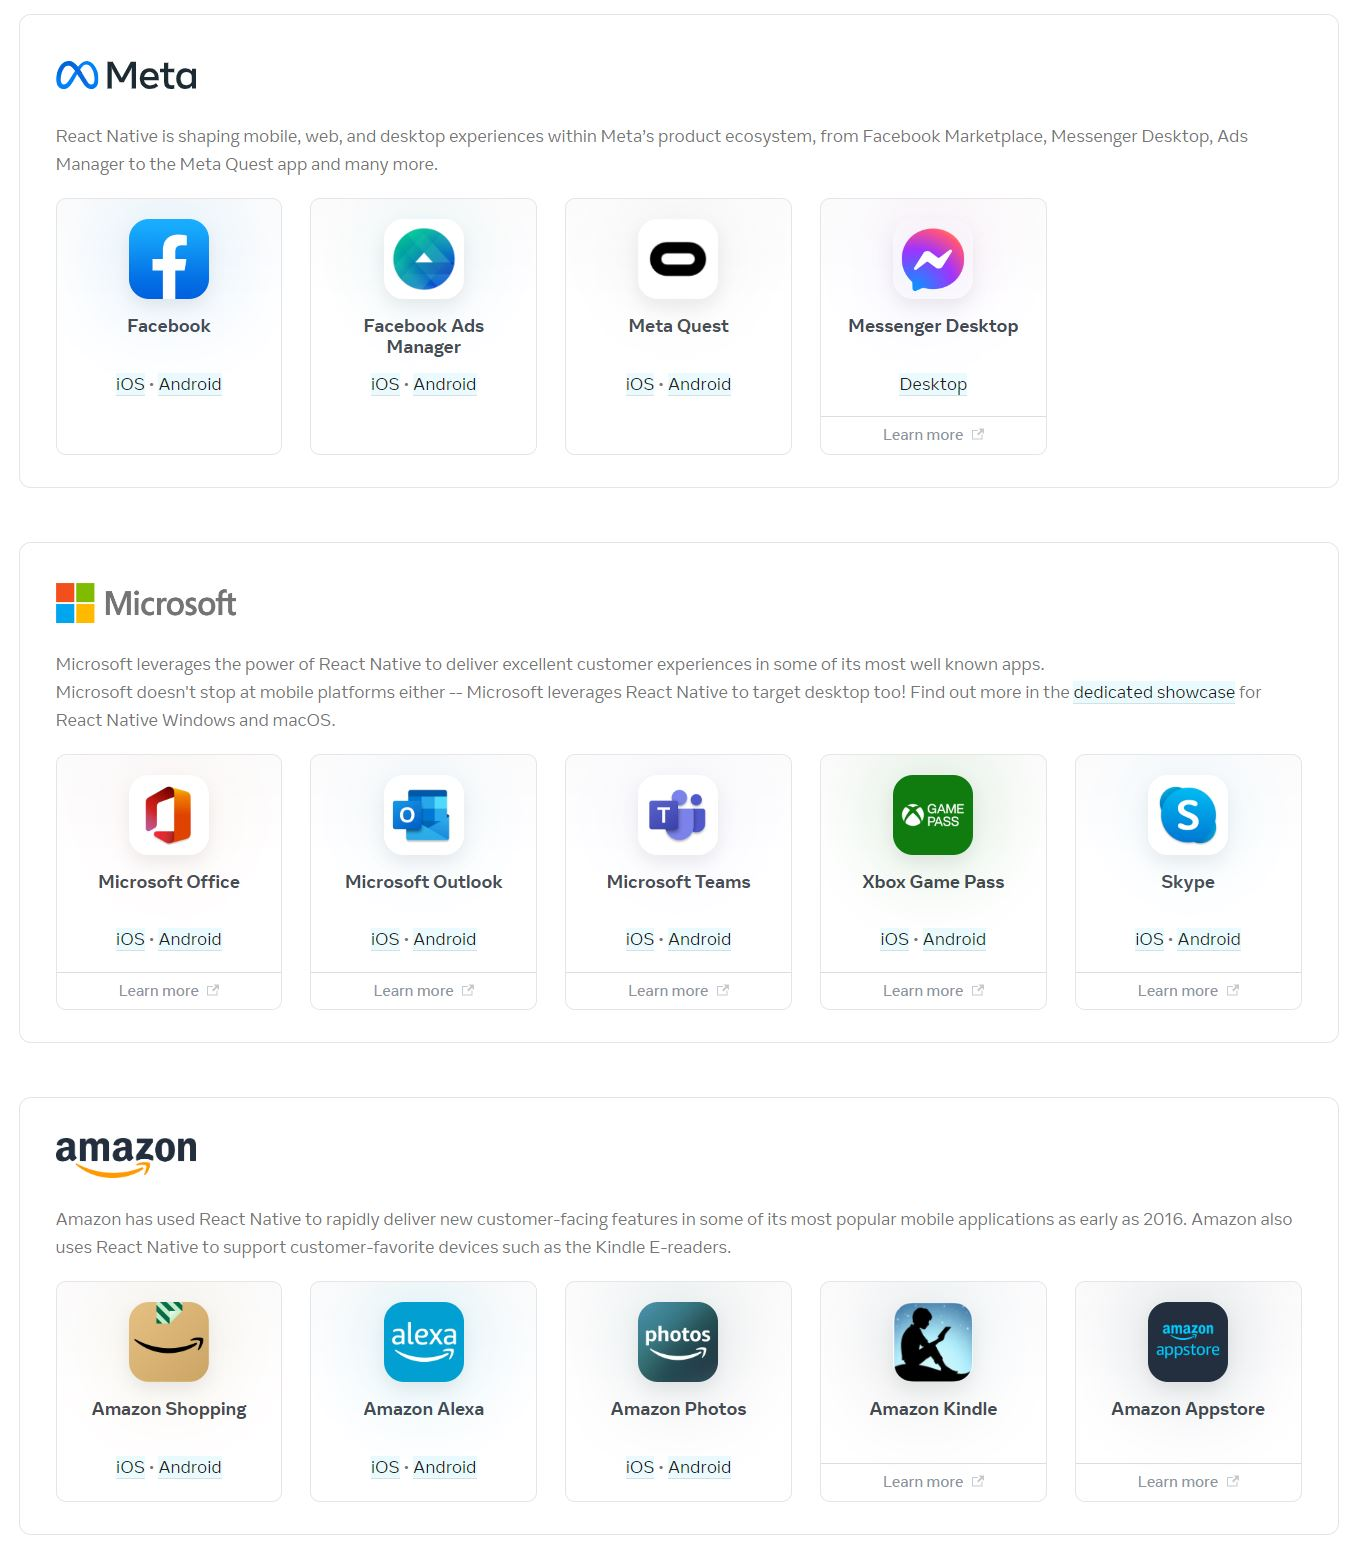
\includegraphics[height=8cm]{Showcase1.JPG}
	\end{frame}
	\subsubsection{0.2.2. Showcase Otras Apps}
	\begin{frame}
		\centering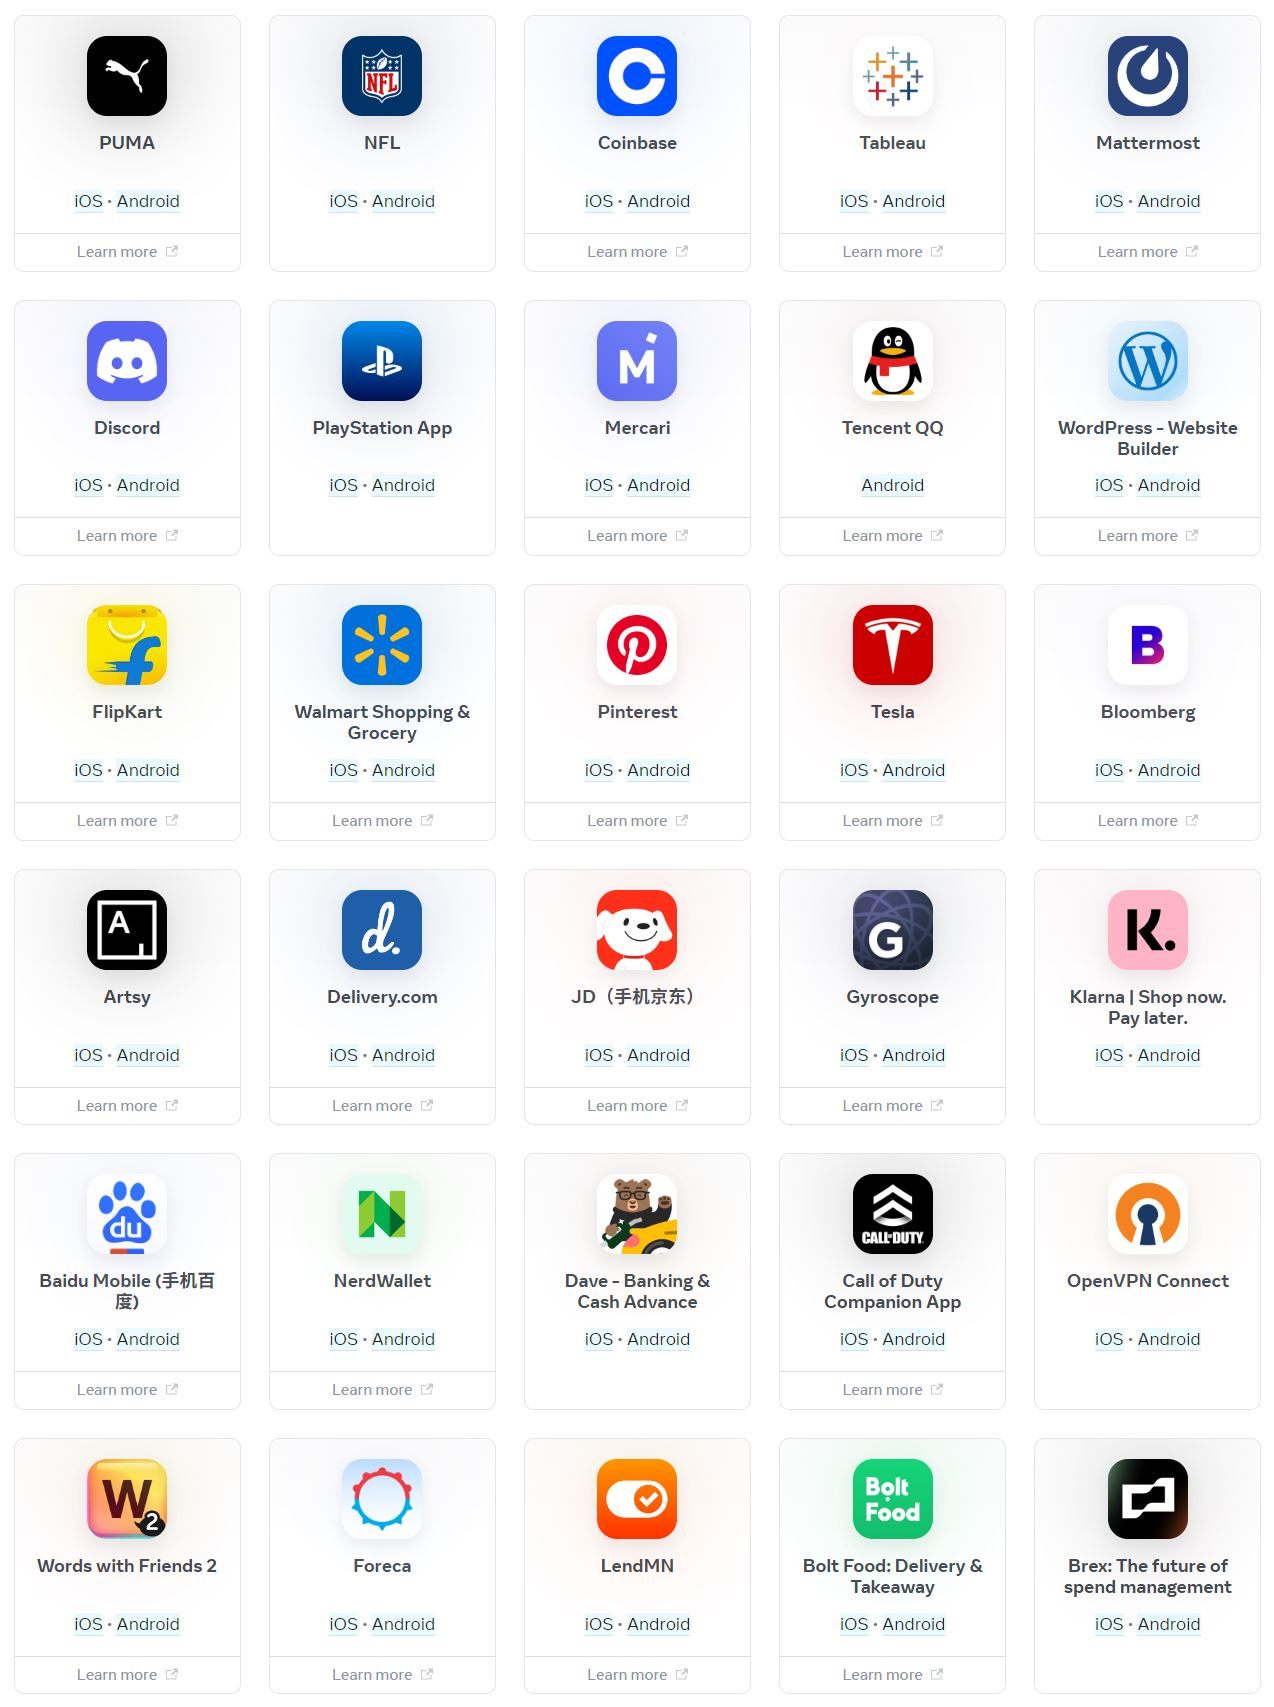
\includegraphics[height=8cm]{Showcase2.JPG}
	\end{frame}
	\section{1. Instalació de React Native}
	\subsection{}
	\subsubsection{}
	\begin{frame}
	\end{frame}
	\
\end{document}
